% Copyright (C) 2005-2015 Airbus - EDF - IMACS - Phimeca
% Permission is granted to copy, distribute and/or modify this document
% under the terms of the GNU Free Documentation License, Version 1.2
% or any later version published by the Free Software Foundation;
% with no Invariant Sections, no Front-Cover Texts, and no Back-Cover
% Texts.  A copy of the license is included in the section entitled "GNU
% Free Documentation License".
\renewcommand{\filename}{docUC_InputBayesian.tex}
\renewcommand{\filetitle}{UC : Creation of a random vector with random parameters}

% \HeaderNNIILevel
% \HeaderIILevel
\HeaderIIILevel



\index{Distribution!Bayesian}
\index{Bayesian! Distribution}

The objective of this Use Case is to create a random vector $\vect{X}$ which distribution $\cL_{\vect{X}|\vect{\Theta}}$ which parameters $\vect{\Theta}$ form a random vector distributed according to the distribution  $\cL_{\vect{\Theta}}$.\\

Note that the random parameters vector $\vect{\Theta}$ is a {\itshape RandomVector} object. We only need its capacity to generate realisations.  It can be :
\begin{itemize}
\item a {\itshape UsualRandomVector} which means described by a given distribution $\cL_{\vect{\Theta}}$;
\item or a {\itshape CompositeRandomVector} which means the output vector of a fonction $f$ evaluated on the random vector $\vect{Y}$  : $\vect{\Theta} = f(\vect{Y})$. In that case, the distribution $\cL_{\vect{\Theta}}$ is a not explicitely known;
\item other complex structures as {\itshape PythonRandomVector, FunctionalChaosRandomVector, Event} \dots.
\end{itemize}

To generate a realization of such a random vector $\vect{X}$, OpenTURNS first generates a realization $\vect{\theta}$  of the random vector  $\vect{\Theta}$ according to  $\cL_{\vect{\Theta}}$, then a realization of the distribution $\cL_{\vect{X}|\vect{\Theta}=\vect{theta}}$.\\


\requirements{
  \begin{description}
  \item[$\bullet$] the distribution $\cL_{\vect{X}|\vect{\Theta}}$: {\itshape myX\_ThetaDist}
  \item[type:] Distribution
  \item[$\bullet$] the distribution $\cL_{\vect{\Theta}}$: {\itshape myThetaDist}
  \item[type:] Distribution
  \item[$\bullet$] the function $f$: {\itshape model}
  \item[type:] NumericalMathFunction
  \item[$\bullet$] the input random vector $\vect{Y}$: {\itshape inputYRV}
  \item[type:] RandomVector
  \end{description}
}
{
  \begin{description}
   \item[$\bullet$] the random vector $\vect{\Theta}$: {\itshape myThetaRV\_1, myThetaRV\_2}
  \item[type:]  RandomVector (of type Usual or Composite)
  \item[$\bullet$] the random vector $\vect{X}$: {\itshape X\_1,X\_2}
  \item[type:]  ConditionalRandomVector
   \item[$\bullet$] the distribution of $\vect{X}$ given $\vect{\Theta}$:  {\itshape Xdist }
  \item[type:] Distribution
  \item[$\bullet$] a random vector: {\itshape rdTheta}
  \item[type:] RandomVector
  \end{description}
}

\textspace\\
Python script for this UseCase :

\inputscript{script_docUC_InputBayesian_RandomVector}

\textspace\\

The following example illustrates a scalar random vector $X$ distributed according to a Normal distribution: $\cL_{\vect{X}|\vect{\Theta}=(M, \Sigma)} = Normal(M, \Sigma)$, wich parameters are defined by:
\begin{itemize}
\item $M \sim Uniform([0,1])$,
\item $\Sigma \sim Exponential(\lambda=4)$.
\end{itemize}

The figure Fig.\ref{DensitCond} draws the probability density function of $X$ that has been built with the kernel smoothing technique from $n=10^6$ realizations of $X$ with the normal kernel. It also draws, for comparison needs, the probability density function of $X$ in the case where the parameters are fixed to their mean value.\\

\begin{figure}[H]
  \begin{center}
    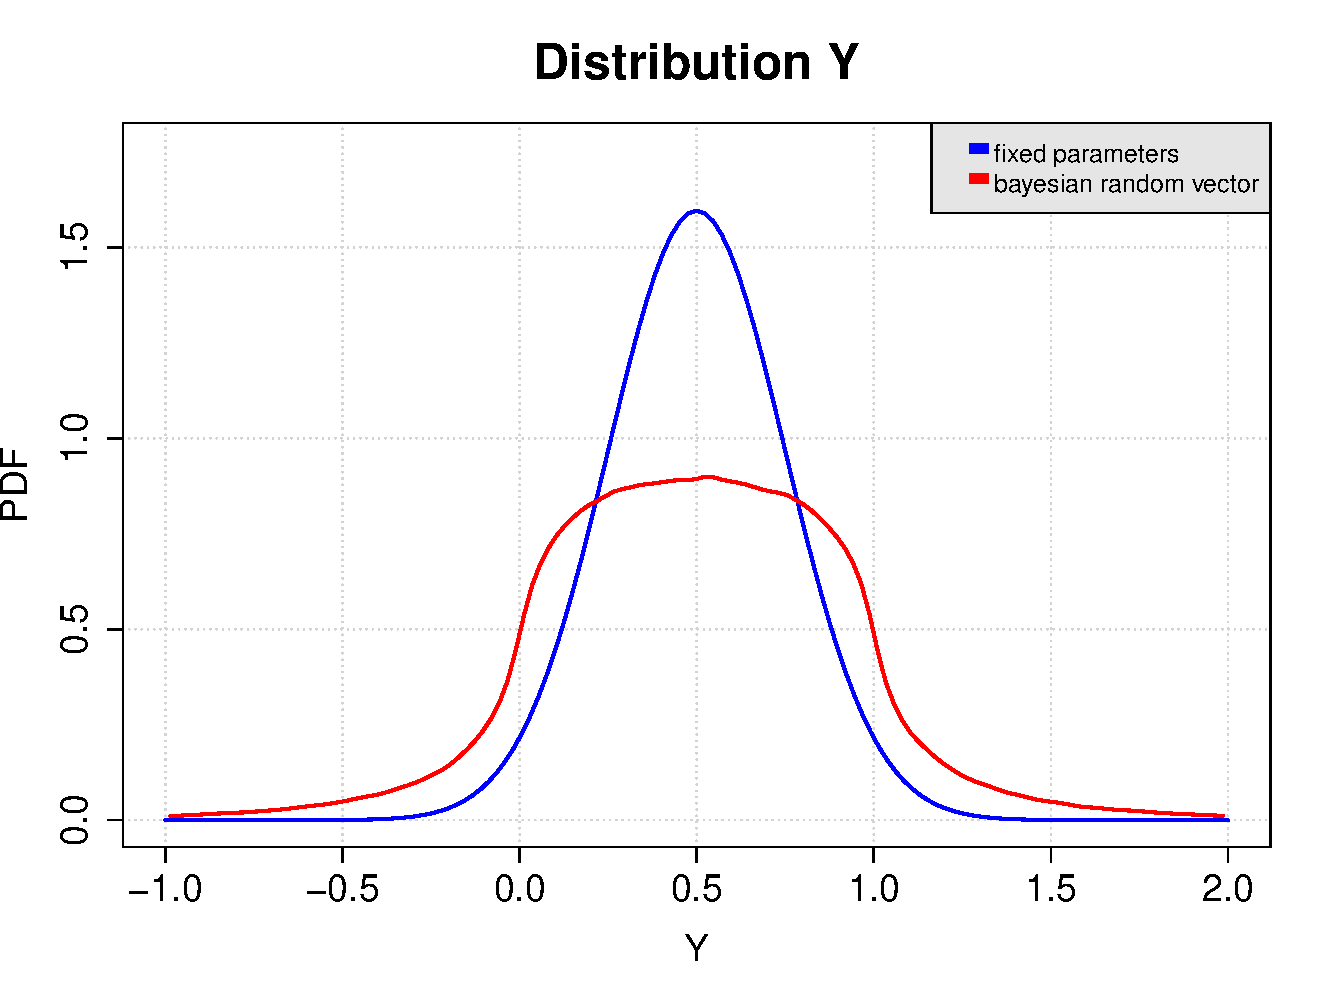
\includegraphics[width=7cm]{Figures/pdf_bayesianRandomVector.pdf}
    \caption{Normal distribution with random or fixed parameters.}
    \label{DensitCond}
  \end{center}
\end{figure}

Besides, if we consider the event $\cE = \{X > 1.5\}$, we have $\Prob{\cE}= 1.75\, e-2$ in the first case of random parameters and $\Prob{\cE}= 3.17\, e-5$ in the case of fixed parameters.\\

Note that we can compare both models using {\itshape ConditionalRandomVector} and {\itshape ConditionalDistribution} objects. We recall that $\vect{X}_{\vect{\Theta}} \sim \cL_{\vect{X}|\vect{\Theta}}$ and $\vect{\Theta} \sim \cL_{\vect{\Theta}}$, where
$\cL_{\vect{X}|\vect{\Theta}}$ and $\cL_{\vect{\Theta}}$ are {\itshape Distribution} objects, $\vect{\Theta}$ is a {\itshape RandomVector} object.\\

Using the {\itshape ConditionalRandomVector} object, we can model $\vect{X}$ as follows:
\begin{align*}\label{CondRV}
  \vect{X} = ConditionalRandomVector(\cL_{\vect{X}|\vect{\Theta}}, \vect{\Theta})
\end{align*}
This model enables to generate realizations of $\vect{X}$ but does not give access to its distribution.\\
According to the way the random vector $\vect{\Theta}$ has been modeled, we can use other equivalent models:
\begin{itemize}
\item $\vect{\Theta}$ is a {\itshape UsualRandomVector}, defined by its {\itshape Distribution} $\cL_{\vect{\Theta}}$:
  \begin{align*}
    \vect{\Theta} = RandomVector(\cL_{\vect{\Theta}})
  \end{align*}
  Then (\ref{CondRV}) is equivalent to:
  \begin{align}\label{CondDist1}
    \vect{X} = RandomVector(ConditionalDistribution(\cL_{\vect{X}|\vect{\Theta}}, \cL_{\vect{\Theta}}))
  \end{align}
  Here we have the fact that by default, the link function is the identity one.

\item $\vect{\Theta}$ is a {\itshape CompositeRandomVector}, defined by $\vect{\Theta} = f(\vect{Y})$, where $\vect{Y}$ is a {\itshape UsualRandomVector},
  defined by its distribution $\cL_{\vect{Y}}$:
  \begin{align*}
    \vect{Y} = & RandomVector(\cL_{\vect{Y}})\\
    \vect{\Theta} = & RandomVector(f, \vect{Y})
  \end{align*}
  Then (\ref{CondRV}) is equivalent to:
  \begin{align}\label{CondDist2}
    \vect{X} = RandomVector(ConditionalDistribution(\cL_{\vect{X}|\vect{\Theta}}, \cL_{\vect{Y}}, f))
  \end{align}
  If $\vect{\Theta}$ and $\vect{Y}$ are of dimension 1, then we can use the {\itshape CompositeDistribution} object to define the distribution $\cL_{\vect{\Theta}}$ as follows:
  \begin{align}\label{CondDist3}
    \vect{X} = RandomVector(ConditionalDistribution(\cL_{\vect{X}|\vect{\Theta}}, CompositeDistribution(f,\cL_{Y}))
  \end{align}

\end{itemize}
Note that all the modellings (\ref{CondDist1}), (\ref{CondDist2}) and (\ref{CondDist3}) give access to the final distribution of $\vect{X}$ and thus enable to use all the methods inherent to a {\itshape Distribution} object, such as {\itshape computeMean(), \dots}.